\documentclass[12pt,a4paper]{article}
\usepackage[utf8]{inputenc}
\usepackage[left=2.5cm,right=2.5cm,top=3cm,bottom=2cm]{geometry}
\author{Pauline Speckmann}
\usepackage{graphicx}
\usepackage{booktabs}

\usepackage{fancyhdr}
\pagestyle{fancy}
\fancyhf{}
\fancyhead[l]{Digitalisierung Vorlesung 4 $-$ Zusammenfassung von Pauline Speckmann}
\fancyhead[r]{\thepage}

\begin{document}
\setcounter{section}{3}
\section{Konzept der digitalen Transformation}


\vspace*{1cm}
\subsection{Grundlagen digitale Transformation} %%%%%%%%%%%%%%%%%%%%%%%%%%%%%%%%%%%%%%%%%%%%%%%%%%%%%%%%%%%%%%%%%%%%%%%%%%%%%%%%%
\begin{itemize}
   \item \textbf{Potenziale von IT - Traditionelle Perspektive}
      \begin{itemize}
			\item Unstrukturierte Abläufe in routinemäßige Arbeit überführen
			\item Beschleunigung wertschöpfender Aktivitäten
			\item Ersatz und Reduktion menschlicher Arbeit
			\item Transport von Informationen mit großer Geschwindigkeit über große Entfernungen
			\item Große Menge von Informationen verfügbar machen
      \end{itemize}

   \item \textbf{Unternehmensstrategie und Informationssysteme}:
   \item[] 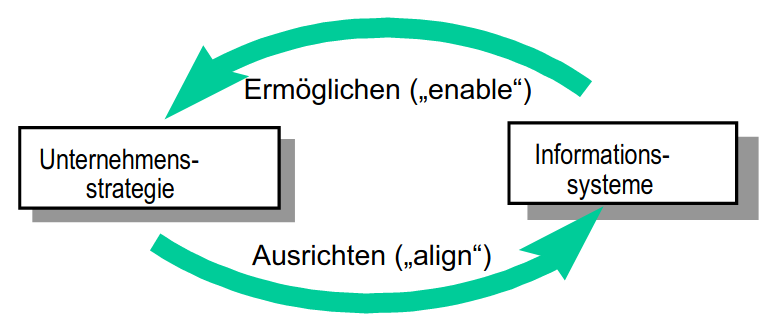
\includegraphics[scale=0.45]{UIS.png}
   
   \item \textbf{Potenziale digitaler Technologien für die Wertschöpfung}:
   \item[] 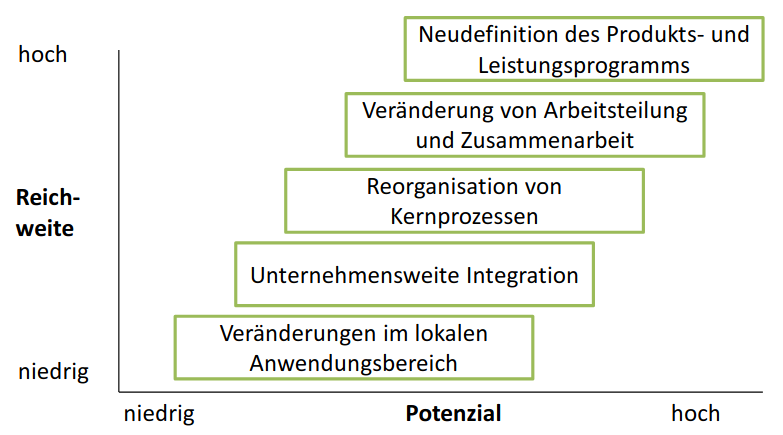
\includegraphics[scale=0.5]{Potenziale.png}
   
   \item \textbf{Digitale Transformation - Zentrale Schritte}:
      \begin{itemize}
			\item \textbf{Starke operationale Grundlage}: \\
			      Zuverlässige Kunden- und Produktdaten, End-to-End Transaktionsprozesse, Transparenz bei Kundentransaktionen
			\item \textbf{Experimentierfreudigkeit}: \\
			      Umfassende Einbindung von Mitarbeiter in Innovationsbemühungen
			\item \textbf{Datengesteuerte Entscheidungskultur}: \\
			      Hypothesenbildung, Datensammlung und detaillierte Auswertung, Top-Level Entscheidungskultur
			\item \textbf{Digitale Angebotsplattform}: \\
			      Wiederverwendbare Datentools und Algorithmen, Unterstützung bei der Konfiguration digitaler Lösungen
      \end{itemize}
\end{itemize}


\vspace*{0.5cm}
\subsection{Digitale Technologie: Treiber der digitalen Transformation} %%%%%%%%%%%%%%%%%%%%%%%%%%%%%%%%%%%%%%%%%%%%%%%%%%%%%%%%%
\begin{itemize}
   \item Cloud Computing (Wiederholung von VL3)
   \item[] 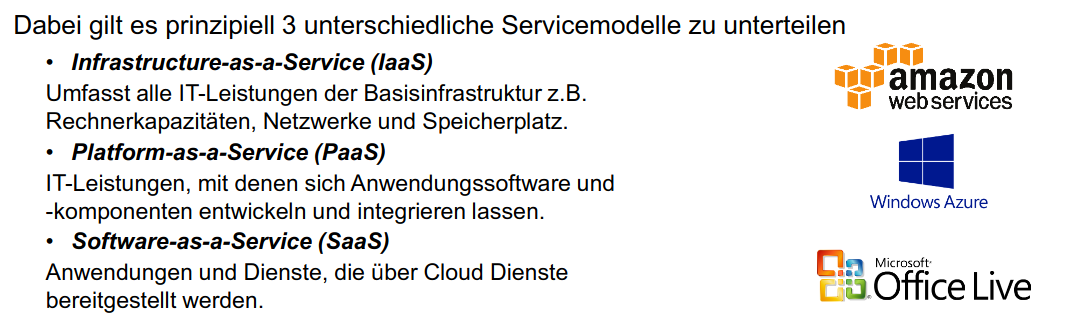
\includegraphics[scale=0.4]{repeat.png}
   \item[] \hspace*{0.5cm} 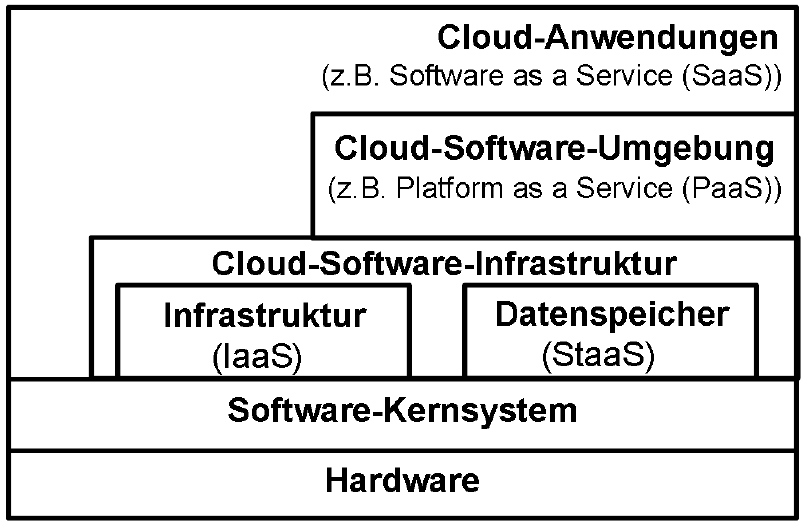
\includegraphics[scale=0.3]{CloudComputingKonzept.png}
   
   \item \textbf{Internet of Things}:\\
         Erweitertes Internet, in dem neben klassischen Rechnern und mobilen Endgeräten auch beliebige physische Gegenstände eingebunden werden

   \item \textbf{Augmented Reality}:
      \begin{itemize}
			\item Erweiterte Realität\\
			      Computergestützte Erweiterung der Realitätswahrnehmung
			\item Beispiel: mit App und Kamera Möbel virtuell in physischem Zimmer platzieren
      \end{itemize}

   \item \textbf{Blockchain}:
      \begin{itemize}
			\item Elektronisches Register (Liste) von Datensätzen (verteilte, öffentliche Datenbank)
			\item Dezentral verwaltet $\rightarrow$ sicher
			\item Blöcke (neue mit alten) werden unveränderbar miteinander verkettet
      \end{itemize}

   \item \textbf{Kerneigenschaften digitaler Technologien}:
      \begin{itemize}
			\item Homogenität der Daten:\\
			      Verschiedene Dateiformate können für verschiedene Zwecke genutzt werden
			\item Re-Programmierbarkeit:\\
			      Technologie kann für verschiedene Zwecke eingesetzt werden
			\item Selbstreferenzierung:\\
			      z.B. Kindle nutzt die Amazon Cloud zum Speichern der Bücher wodurch abhängige Netzwerkeffekte zu digitalen Innovation entstehen
      \end{itemize}
\end{itemize}


\vspace*{0.5cm}
\subsection{Wertschöpfungsstrukturen verändern} %%%%%%%%%%%%%%%%%%%%%%%%%%%%%%%%%%%%%%%%%%%%%%%%%%%%%%%%%%%%%%%%%%%%%%%%%%%%%%%%%
\begin{itemize}
   \item \textbf{Veränderungen von Wertschöpfung durch digitale Transformation}:
   \item[] 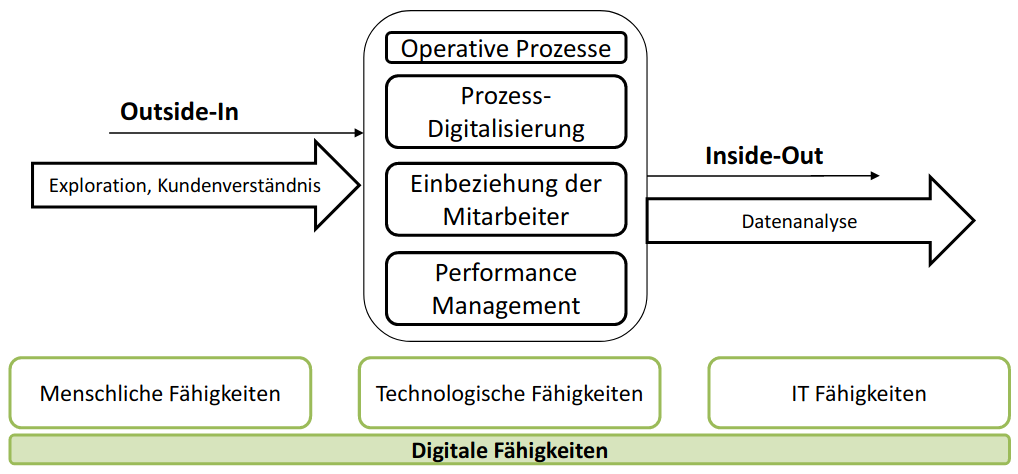
\includegraphics[scale=0.40]{veraenderung.png}
   
   \item \textbf{Digitale Fertigkeiten eines Unternehmens}:\\
         Digitale Daten und Informationstechnologien in seine Produkte, Dienstleistungen, Geschäftsprozesse und organisatorischen Systeme zu integrieren und so einen Mehrwert zu generieren
		\begin{itemize}
			\item IT-Unternehmenspartnerschaften
			\item Externe IT-Verbindungen
			\item Strategische Ausrichtung der IT
			\item IT Geschäftsprozessintegration
			\item IT Management
			\item IT Infrastruktur
		\end{itemize}

   \item \textbf{Wechselwirkung Produzent $–$ Konsument}:
   \item[] 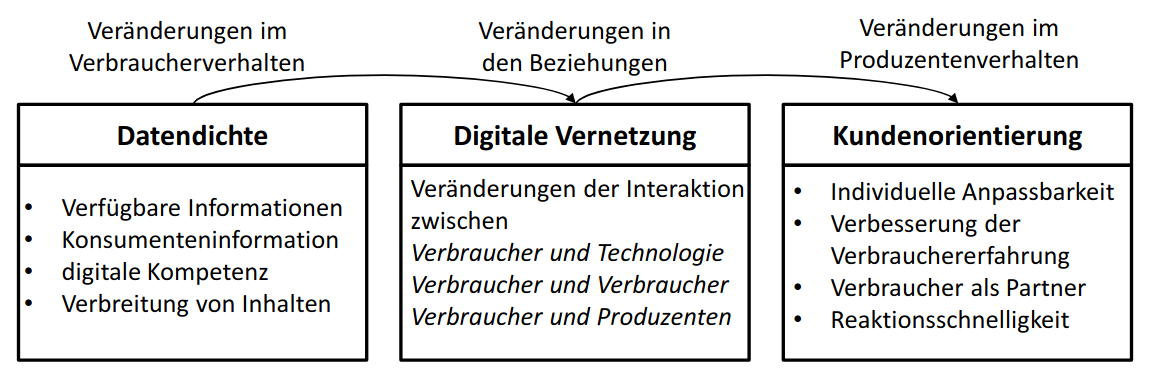
\includegraphics[scale=0.33]{prozess.png}
   
   \item \textbf{Modulare Architekturen}:\\
         Aufteilung eines Produktes in möglichst unabhängige Module (Verbund über standardisierte Schnittstellen)\\
         $\rightarrow$ Flexibilität
         
   \item \textbf{Consumerization}:
      \begin{itemize}
			\item Definition aus Vorlesung: \\
			Consumerization bezeichnet den spezifischen Einfluss, den verbraucherorientierte Technologien auf Unternehmen haben können. Sie spiegelt wider, wie Unternehmen von neuen Technologien und Modellen, die aus dem Konsumbereich und nicht aus dem Unternehmens-IT-Sektor stammen, beeinflusst werden und diese nutzen können.
			\item Wikipedia: \\
			Consumerization bezeichnet den Prozess bzw. die Erscheinung, dass elektronische Endgeräte, wie beispielsweise Smartphone, Tablet-PCs, von Arbeitnehmern auch für ihre Erwerbsarbeit benutzt werden.
      \end{itemize}
      

   \begin{minipage}[t]{0.4\textwidth}

	\textbf{Vorteile Consumerization} 
	\begin{itemize}
	\item bestimmte Arbeiten lassen sich dezentralisieren und flexibler organisieren und durchführen
	\item mehr Kontrolle der Arbeitnehmer über ihre Zeit und Arbeitsbeziehungen
	\end{itemize}

\end{minipage}\begin{minipage}[t]{0.1\textwidth}
   \ 
\end{minipage}\begin{minipage}[t]{0.4\textwidth}

	\textbf{Nachteile Consumerization} 
	\begin{itemize}
	\item auflösende Grenze zwischen Berufs- und Privatleben
	\item geringere Kontrollmöglichkeiten der Unternehmen
	\item Firmen können über die Netzwerkverbindungen auf die privat genutzten Geräte zugreifen
	\item Sicherheitsprobleme
	\end{itemize}


\end{minipage}
\end{itemize}



\newpage
\subsection{QUIZFRAGEN} %%%%%%%%%%%%%%%%%%%%%%%%%%%%%%%%%%%%%%%%%%%%%%%%%%%%%%%%%%%%%%%%%%%%%%%%%%%%%%%%%%%%%%%%%%%%%%%%%%%%%%%%%%%%%%
\begin{itemize}
   \item Datenbasierte Verfahren sind auf dem Vormarsch.
   \item KI stellt eine neue Anforderung an die Widerstandsfähigkeit von Unternehmen gegen Fehler, was meint, dass:\\
         $\rightarrow$ Das KI-System ist nicht fehlerfrei. Dementsprechend muss das Unternehmen mit einer gewissen Anzahl an Fehlern rechnen/leben können.\\
         $\rightarrow$ Gerade bei neuen KI-Systemen werden Mitarbeiter Fehler in der Anwendung machen. Diese müssen einkalkuliert und toleriert werden.
   \item KI-Systementwicklungsprojekte unterscheiden sich von traditionellen Systementwicklungsprojekten durch eine intensivere initiale Auseinandersetzung mit der Unternehmenssituation, um eine passende KI-Lösung zu finden.
   \item Machine Learning gehört nicht zur schwachen KI Richtung.
   
   \item Software-as-a-Service (SaaS) hat die Vorteile der hohen Transparenz und Flexibilitaet bei den Kosten und der hohen Skalierbarkeit, da SaaS Zugänge schnell an den aktuellen Nutzerzahlen angepasst werden können.
   
   \item Mathematische Verfahren machen die Daten in der Blockchain zuverlässig und vertrauenswürdig und da die Datenbank verteilt ist, ist ein Ausfall des Netzwerks nahezu unmöglich.
   
   \item Ziel der digitalen Transformation ist es durch intensive Experimente neue Geschäftsmodelle zu kreieren.
   
   \item Die Reprogrammierbarkeit als Kern-Eigenschaft einer digitaler Technologien bedeutet, dass verschiedene Funktionen von einem einzigen digitalen Gerät ausgeführt werden können.
   \item Durch die Reprogrammierbarkeit kann ein digitales Gerät eine Vielzahl von Funktionen ausführen (z.B. Textverarbeitung, Videobearbeitung und Web-Browsing).
   \item Die Selbst-Referenzierbarkeit als Kern-Eigenschaft einer digitaler Technologie bedeutet, dass digitale Innovation den Einsatz digitaler Technologien erfordern.
   \item Homogenisierung von Daten bedeutet, dass alle digitalen Inhalte mit den gleichen digitalen Geräten und Netzwerken gespeichert, übertragen, verarbeitet und angezeigt werden können.
   
   \item Das Internet der Dinge bezeichnet die Verbindung von Gegenständen mit dem Internet, damit diese Gegenstände selbstständig über das Internet kommunizieren können.
   
   \item Der Mensch spielt in der gegenseitigen Beeinflussung von Organisation und IT nur eine untergeordnete Rolle, denn der Zusammenhang zwischen Organisation und IT ist direkt.
   
   \item Die Implementierung voneinander getrennter Business- und IT-Abteilungen ist keine digitale Fähigkeit.
   
   \item Bestandteile der Definition von \emph{Digitale Transformation} sind die Auswirkungen auf Aspekte der Wirtschaft und der Gesellschaft und die Nutzung von Digitalen Innovationen.
\end{itemize}

\end{document}